\chapter{Statistical methods}\label{ch:stat}

In the course of analyzing the data sets provided by the CMS experiment and used in this thesis, several statistical tools have been employed; in this chapter, a description of these tools will be presented, starting with the general statement of the multivariate analysis method, followed by the particularities of the Boosted Decision Trees (BDT) method and its application to the classification problem. Statistical inference methods used will also be presented. This chapter is based mainly on the reference \cite{mva}.      

\section{Multivariate analysis}

Multivariate data analysis (MVA) makes reference to statistical techniques that analyze data containing information of more than one variable, commonly taking into account the effects of all variables on the response of the particular variable under investigation, \ie, considering all the correlations between variables. MVA is employed in a variety of fields like consumer and market research, quality control and process optimization. From a MVA it is possible to identify the dominant patterns in the data, like groups, outliers and trends, and determine to which group a set of values belong; in the particle physics context, MVA methods are used to perform the selection of certain type of events, from a large data set, using a potentially large number of measurable properties for each event.

Processes with small cross section, as the \tHq process, normally are hidden behind more common processes; therefore, the data set results in a subset of events with characteristic features of interest (signal) mixed in randomly with a much larger number of SM events that can mimic these features of interest (background) which implies that it is not possible to say with certainty that a given event is signal or background. In that sense, the problem can be formulated as one where a set of events have to be classified according to some features; these features correspond to the measurements of several parameters like energy, momentum organized in a set of ``input variables''. The measurements for each event can be written in a vector $\textbf{x}=(x_1,.....,x_n)$ for which

\begin{itemize}
\item Signal hypotheses $\to f(\textbf{x}|s)$ is the probability density (``likelihood'') for $\textbf{x}$ given it is a signal event 
\item Background hypotheses $ \to f(\textbf{x}|b)$ is the probability density (``likelihood'') of $\textbf{x}$ given it is a background event
\end{itemize}

Figure \ref{fig:scatter_plot} shows three ways to perform a classification of events for which measurements of two properties, two input variables, have been performed; blue circles represent signal events while red triangles represent background events. The classification on (a) is ``cut-based'' requiring $x_1<c_1$ and $x_2<c_2$; usually the cut values are chosen according to some knowledge about the event process. In (b), the classification is performed by stating a cut involving a linear function of the input variables and so the boundary, while in (c) the the relationship between the input variables is not linear thus the boundary is not linear either.          

\begin{figure}[!h]
  \centering
  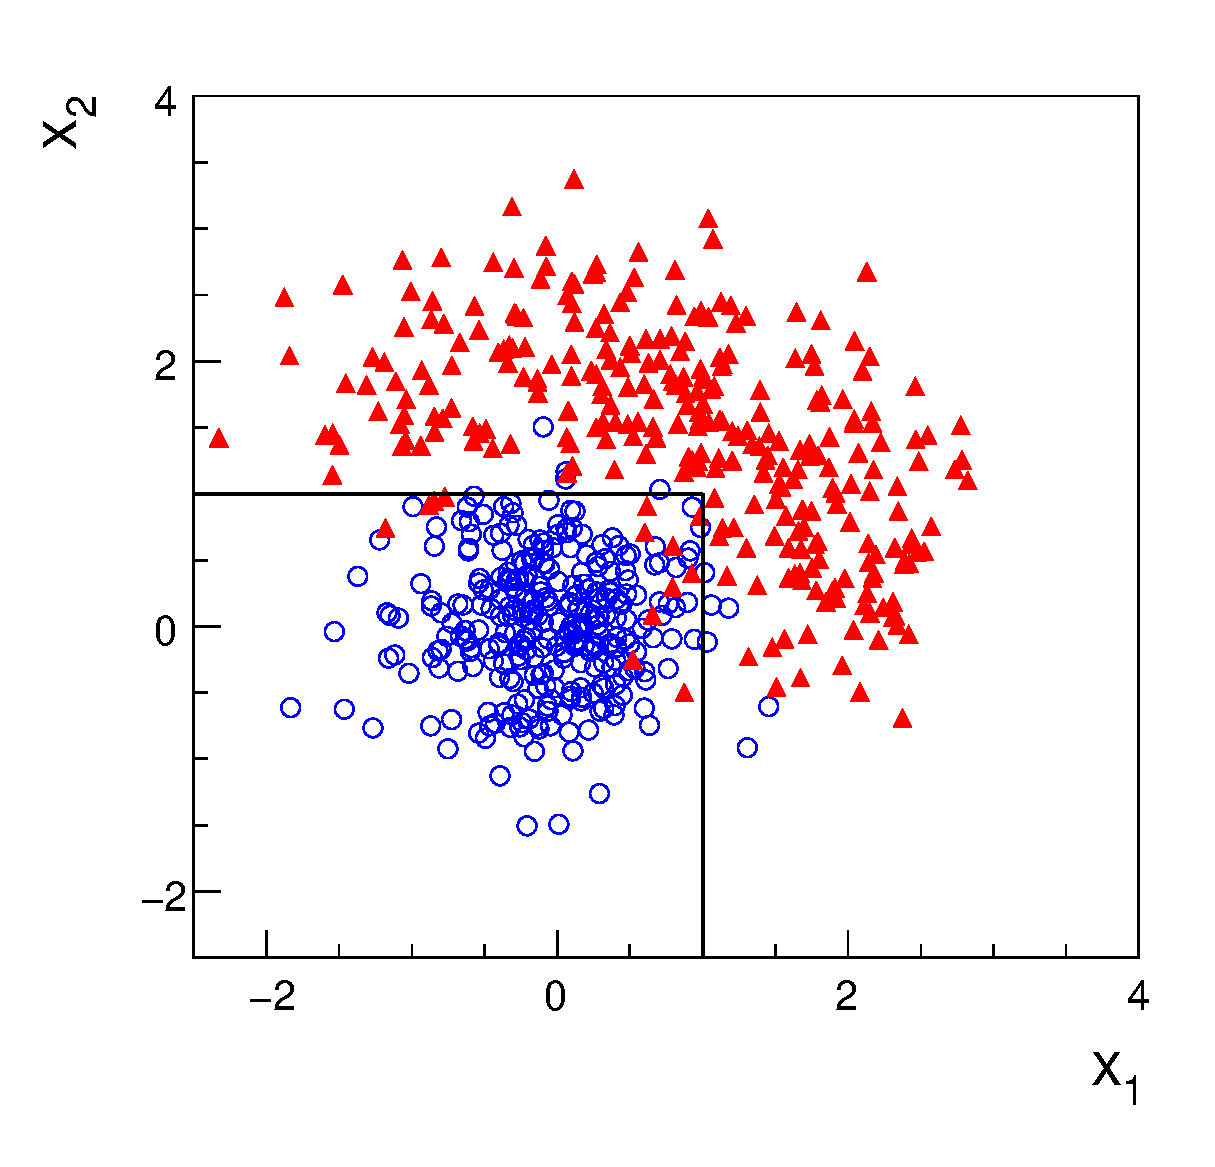
\includegraphics[width=4.5cm,height=4.5cm]{Cuts}
  \includegraphics[width=4.5cm,height=4.5cm]{Fisher}
  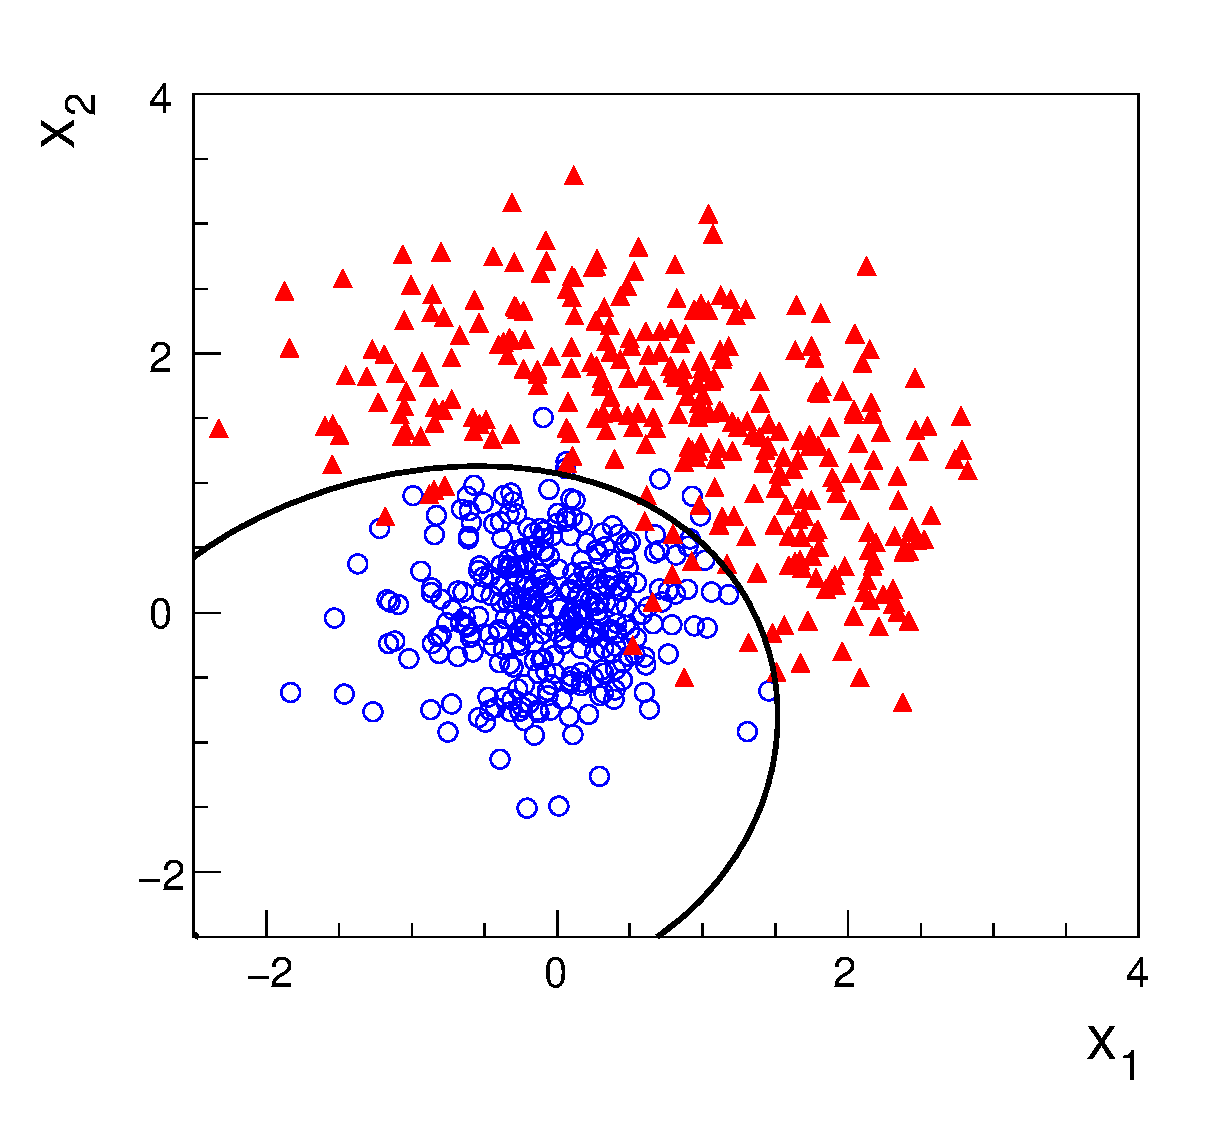
\includegraphics[width=4.5cm,height=4.5cm]{SVM05}
  \caption[Scatter plots-MVA event classification.]{Scatter plots-MVA event classification. Distribution of two input variables $x_1$ and $x_2$ measured for a set of events; blue circles represent signal events and red triangles represent background events. The classification is based on (a) cuts, (b) linear boundary, and (c) nonlinear boundary\cite{mva}}\label{fig:scatter_plot}
\end{figure}

The boundary can be parametrized in terms of the input variables such that the cut is set on the parametrization instead of on the variables, \ie, $y(\textbf{x})=y_{cut}$ with $y_{cut}$ a constant; thus, the acceptance or rejection of an event is based on what side of the boundary is the event located. If $y(\textbf{x})$ has functional form, it can be used to determine the probability distribution functions $p(y|s)$ and $p(y|b)$ and then perform a scalar test statistic with a single cut on the scalar variable $y$. 

\begin{figure}[!h]
  \centering
  \includegraphics[scale=0.4]{TestStat}
  \caption[Scalar test statistical.]{Distributions of the scalar test statistic $y(\textbf{x})$ under the signal and background hypotheses.\cite{mva}}\label{fig:scalar_test}
\end{figure}

Figure \ref{fig:scalar_test} illustrates what would be the probability distribution functions under the signal and background hypotheses for a scalar test statistic with a cut on $y$.


\subsection{Boosted decision trees (BDT) }

For this thesis, the implementation of the MVA strategy, described above, is performed through boosted decision trees (BDT). In a simple picture, a decision tree (\dt) classifies events according to their input variables values by setting a cut on each input variable and checking which events are on which side of the cut, just as proposed in the MVA strategy, but in addition, as a machine learning algorithm, \dt s offer the possibility to be trained and then perform the classification efficiently.   

The training process consists in taking MC samples of signal and background events and split them in two parts each; first parts form the training sample which will be used in the \dt training while the second parts form the test sample which will be used for testing the final classifier obtained from the training. Each event has associated a set of input variables $\textbf{x}=(x_1,.....,x_n)$ which serve to distinguish between signal and background events. Pick one variable, say $x_1$, and for each event value of $x_1$ split the training sample into two sets, then, find the splitting value that provides the best classification, \ie, one set mostly made signal events while the other set is mostly made of background events.


Then repeat this
for each variable in turn. Select the variable and splitting
value which gives the best separation. Initially there
was a sample of events at a “node”. Now there are two
samples called “branches”. For each branch, repeat the
process, i.e., again try each value of each variable for the
events within that branch to find the best variable and
splitting point for that branch. One keeps splitting un-til a given number of final branches, called leaves, are
obtained, or until each leaf is pure signal or pure background,
or has too few events to continue. This description
is a little oversimplified. In fact at each stage one
picks as the next branch to split, the branch which will
give the best increase in the quality of the separation. A
schematic of a decision tree is shown in Fig.1, in which
3 variables are used for signal/background separation:
event hit multiplicity, energy, and reconstructed radial
position.
What criterion is used to define the quality of separation
between signal and background in the split? Imagine
the events are weighted with each event having weight
Wi
. Define the purity of the sample in a branch by

where P
s
is the sum over signal events and P
b
is the
sum over background events. Note that P(1 − P) is 0
if the sample is pure signal or pure background. For a
given branch let






A decision trees (DT) is a consist of consecutive binary questions based on a set of input
variables. Depending on the previous answer a different decision has to be taken on the next

node. After a maximal number of nodes, a final verdict is reached depending on the majority of
event class in the occupied endpoint, the leaf.
In the training of Decision Trees the best possible selection criterion for a node is defined by
maximizing the separation gain S between two consecutive nodes. In order to determine the
separation gain, the purity of each leaf has to be determined as

P
s w s
P = P
,
P
s w s + b w b
P
where s,b w s,b are the summed weights of the signal and background events, respectively 1 .
The purity allows for the determination of the Gini index G, a measure of statistical dispersion,
as
n
X
G = * w i + · P · (1 − P ),
, i=1 -
where w i are the normalized weights for each event. The best possible question for the node
can then be determined by maximizing S, given by
S = G father node − G child I − G child II .
As the Gini index has a maximum at P = 0.5 of G = 0.25 (for unweighted events) the maximal
separation gain would also be S = 0.25 for a maximally disperse starting ensemble (G father =
0.25) and two perfectly separated child nodes (G child = 0). Based on the purity after the training,
leafs are either labeled as signal or background leaves.
By using a multitude of slightly altered decision trees and averaging over the predicted outcome
the robustness of the procedure can be ensured, as a badly trained tree due to aberrations does
not have enough power to sway the decision into the wrong direction. The average of all
classifier outputs is later used as a final discrimination variable, labeled as ”BDT output”.


By using the boosting method the full potential of decision trees can be exploited. By sub-
sequently training a multitude of trees, where in each iteration falsely categorized events get
assigned a higher weight, the focus of the training is shifted to classify these previously misiden-
tified events correctly.
In this thesis the AdaBoost [124] algorithm is utilized. Misclassified events are assigned a boost
weight α i for each tree i which is dependent on the misclassification rate Γ i of tree i in the
previous training iteration:
1 − Γ i
α i =
.
Γ i
Correctly classified events get reweighted such that the sum of weights remains constant. The
BDT output of a boosted ensemble of N decision trees is determined as
y Boost (x) =
N
1 X
·
ln α i · h i (x),



where h(x) is the binary outcome of tree i, mathematically realized as h(x) = 1 for events
ending on a signal leaf and h(x) = −1 for events ending on a background leaf.















\section{} 




 Notice that the tails of the distributions indicate that some signal events fall on the rejection region and some background events fall on the acceptance region; therefore, it is convenient to define the ``efficiency'' with which events of a given type are accepted, thus, the signal and background efficiencies are given by 

\begin{eqnarray}
\label{eq:sigeff}
\varepsilon_{\textrm{s}} & = & P( \mbox{accept event} | \mbox{s} ) = \int_{\textrm{A}} f(\textbf{x} | \mbox{s} ) \, d \textbf{x} = \int_{-\infty}^{y_{\textrm{cut}}} p(y | \mbox{s}) \, dy\;, \\*[0.3 cm]
\varepsilon_{\textrm{b}} & = & P( \mbox{accept event} | \mbox{b} ) = \int_{\textrm{A}} f(\textbf{x} | \mbox{b} ) \, d \textbf{x} = \int_{-\infty}^{y_{\textrm{cut}}} p(y | \mbox{b}) \, dy \;,
\end{eqnarray}

where A is the acceptance region. Under these conditions, the background hypothesis corresponds to the ``null hypothesis ($H_0$)'', the signal hypothesis corresponds to the ``alternative hypothesis ($H_1$)'', the background efficiency is the significance level of the test, and signal efficiency is the power of the test; what is sought in an analysis is to maximize the power of the test relative to the significance level.








; it is achieved, according to the Neyman-Pearson lemma\cite{npl},






by defining the acceptance region such that, for $\textbf{x}$ inside the region, the likelihood ratio, i.e., the ratio of probability distribution functions for signal and background,







\section{ MVA methods, NN, BDT, boosting, overtraining, variable ranking  }
\section{statistical inference, likelihood parametrization}
\section{ nuisance parameters}
\section{exclusion limits }
\section{asymptotic limits }


 









